\documentclass[%
aip,
% jmp,
% bmf,
% sd,
% rsi,
amsmath,amssymb,
%preprint,%
reprint,%
%author-year,%
%author-numerical,%
% Conference Proceedings
]{revtex4-1}

\draft % marks overfull lines with a black rule on the right

\usepackage{graphicx}% Include figure files
\graphicspath{{figures/}}
\usepackage{dcolumn}% Align table columns on decimal point
\usepackage{bm}% bold math
%\usepackage[mathlines]{lineno}% Enable numbering of text and display math
%\linenumbers\relax % Commence numbering lines

\usepackage[utf8]{inputenc}
\usepackage[T1]{fontenc}
\usepackage{mathptmx}

\renewcommand{\thefigure}{S\arabic{figure}}

\newcommand{\x}{{\mathbf x}}
\newcommand{\y}{{\mathbf y}}
\newcommand{\etab}{{\mathbf \eta}}

\begin{document}
	
	\preprint{AIP/123-QED}
	
	\title[Supplementary Material: Generalised early warning signal methods]{Supplementary Material: Generalised early warning signals in multivariate and gridded data with an application to tropical cyclones}
	% Force line breaks with \\
	
	\author{J. Prettyman}
	\altaffiliation[Also at ]{National Physical Laboratory}%Lines break automatically or can be forced with \\
	\author{T. Kuna}%
	\affiliation{ 
		University of Reading, Whiteknights, Reading, RG6 6AX, UK%\\This line break forced with \textbackslash\textbackslash
	}%	
	\author{V. Livina}
	\affiliation{%
		National Physical Laboratory, Hampton road, Teddington, TW11 0LW, UK%\\This line break forced% with \\
	}%
	\email{Correspondence to v.livina@npl.co.uk}
	
	\date{\today}% It is always \today, today,
	%  but any date may be explicitly specified






\maketitle

\section*{Sensitivity analysis}

\begin{figure*}
	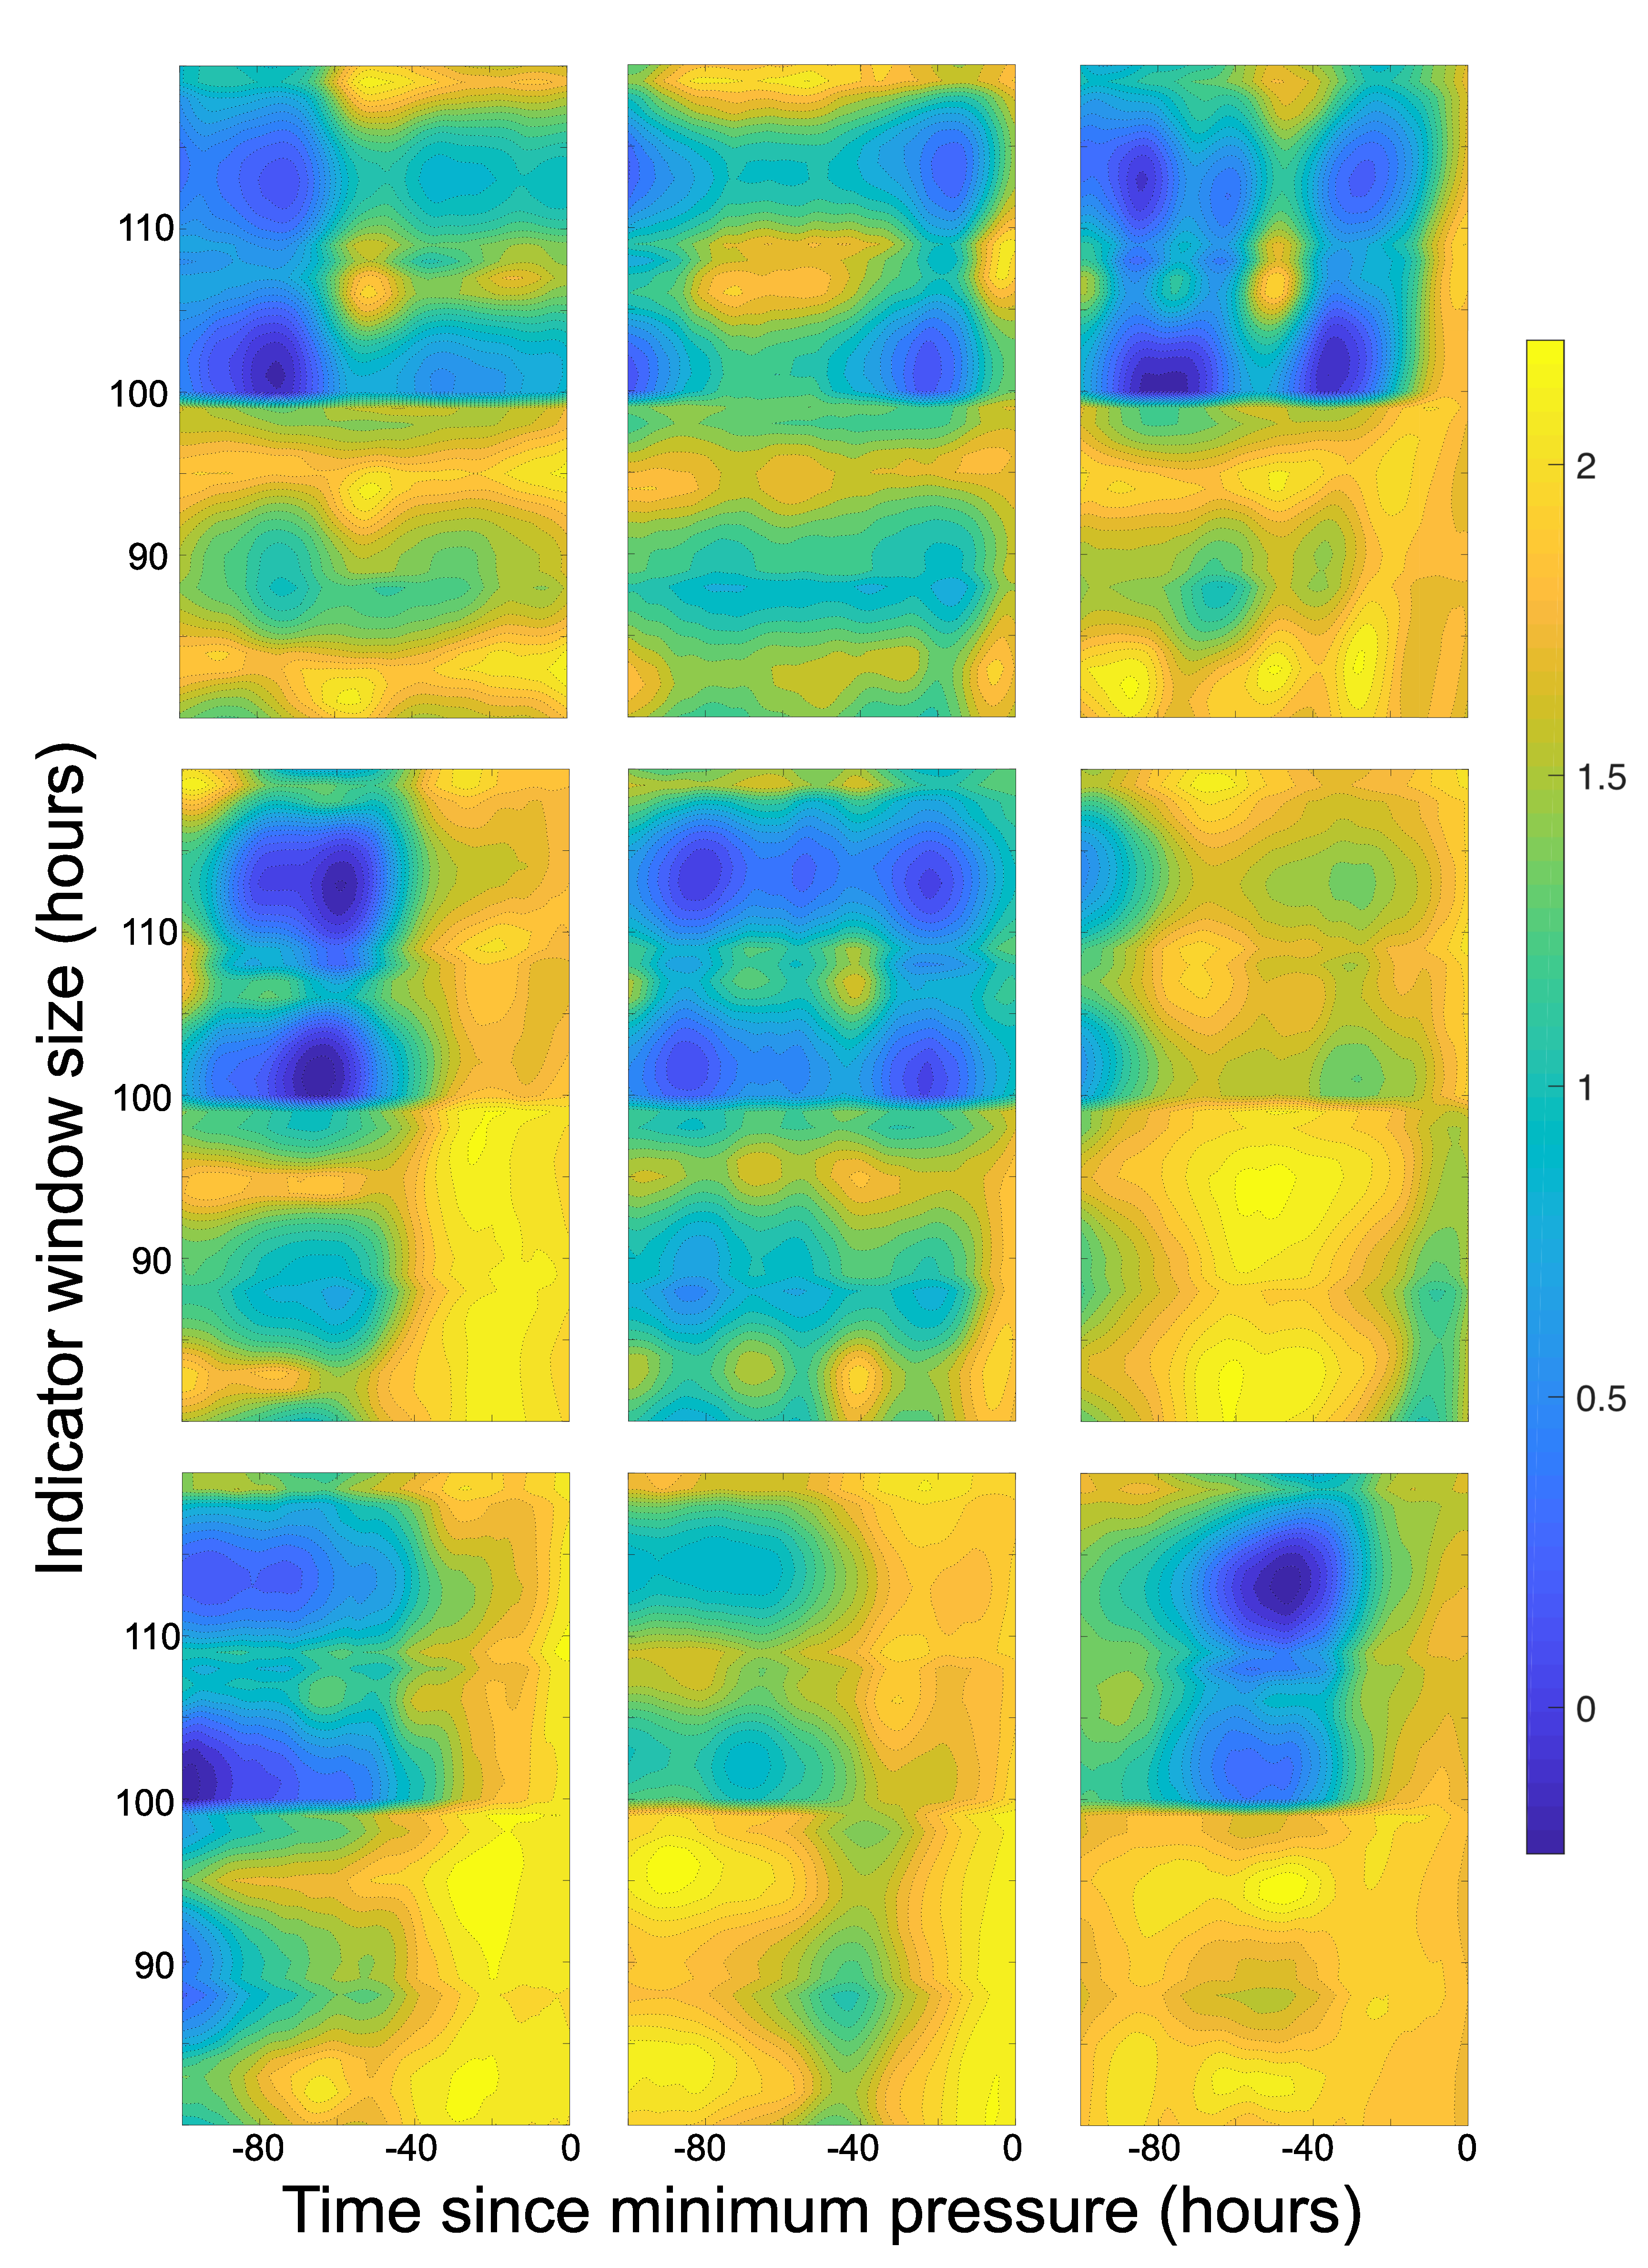
\includegraphics[width=\linewidth]{08_Sensitivity3x3}
	\caption{Sensitivity plots showing the PS-indicator value over time for indicator window sizes in the range $80$ to $120$ points. Left to right: Andrew (Florida); Andrew (Louisiana); Katrina; Wilma; Gustav; Matthew; Harvey; Irma; Nate.}
	\label{fig_Sensitivity3by3}
\end{figure*}

Here we test the sensitivity of the hurricane data to the PS-indicator method by calculating the indicator with a range of sliding window sizes. We hope to use a sliding window of roughly 100 time points (hours) because any longer would mask the indicator signal and a window much shorter than 100 points will introduce too much noise and distort the signal. This has been investigated previously\cite{prettyman2018} and it has been noted that the indicator is strongest when the size of the sliding window is an odd multiple of 6 hours, probably due to tidal oscillations, which is confirmed by our analysis here.

For each of the nine hurricanes, the sea-level pressure series from all stations are aligned about their points of minimum pressure (time zero). The PS-indicator is then applied to all of the time series and the mean is taken. This is performed 41 times, using window sizes in the range $[80,120]$. A smoothing function is then applied to these means which averages each point over the previous 12 hours, this makes it easier to see the necessary detail. The smoothed mean PS-indicators are then plotted over both time and window size as a contour plot. The plots are shown in Fig.~\ref{fig_Sensitivity3by3}. 

These plots allow us to choose a suitable window size for the PS-indicator which will provide the best EWS. In all cases, an indicator window size of either 90 hours or 102 hours was chosen. We can also see from these plots that a time window of 30 to 50 hours before time zero will show the increase in the indicator value most clearly.

We also notice that in every case, there is a qualitative change which happens when the window size is around 100 hours. This occurs even when smoothing is not used and also when the plot only uses data from a single station (rather than the mean over several stations in the region). 

%merlin.mbs aipnum4-1.bst 2010-07-25 4.21a (PWD, AO, DPC) hacked
%Control: key (0)
%Control: author (8) initials jnrlst
%Control: editor formatted (1) identically to author
%Control: production of article title (0) allowed
%Control: page (1) range
%Control: year (1) truncated
%Control: production of eprint (0) enabled
\begin{thebibliography}{1}%
	\makeatletter
	\providecommand \@ifxundefined [1]{%
		\@ifx{#1\undefined}
	}%
	\providecommand \@ifnum [1]{%
		\ifnum #1\expandafter \@firstoftwo
		\else \expandafter \@secondoftwo
		\fi
	}%
	\providecommand \@ifx [1]{%
		\ifx #1\expandafter \@firstoftwo
		\else \expandafter \@secondoftwo
		\fi
	}%
	\providecommand \natexlab [1]{#1}%
	\providecommand \enquote  [1]{``#1''}%
	\providecommand \bibnamefont  [1]{#1}%
	\providecommand \bibfnamefont [1]{#1}%
	\providecommand \citenamefont [1]{#1}%
	\providecommand \href@noop [0]{\@secondoftwo}%
	\providecommand \href [0]{\begingroup \@sanitize@url \@href}%
	\providecommand \@href[1]{\@@startlink{#1}\@@href}%
	\providecommand \@@href[1]{\endgroup#1\@@endlink}%
	\providecommand \@sanitize@url [0]{\catcode `\\12\catcode `\$12\catcode
		`\&12\catcode `\#12\catcode `\^12\catcode `\_12\catcode `\%12\relax}%
	\providecommand \@@startlink[1]{}%
	\providecommand \@@endlink[0]{}%
	\providecommand \url  [0]{\begingroup\@sanitize@url \@url }%
	\providecommand \@url [1]{\endgroup\@href {#1}{\urlprefix }}%
	\providecommand \urlprefix  [0]{URL }%
	\providecommand \Eprint [0]{\href }%
	\providecommand \doibase [0]{http://dx.doi.org/}%
	\providecommand \selectlanguage [0]{\@gobble}%
	\providecommand \bibinfo  [0]{\@secondoftwo}%
	\providecommand \bibfield  [0]{\@secondoftwo}%
	\providecommand \translation [1]{[#1]}%
	\providecommand \BibitemOpen [0]{}%
	\providecommand \bibitemStop [0]{}%
	\providecommand \bibitemNoStop [0]{.\EOS\space}%
	\providecommand \EOS [0]{\spacefactor3000\relax}%
	\providecommand \BibitemShut  [1]{\csname bibitem#1\endcsname}%
	\let\auto@bib@innerbib\@empty
	%</preamble>
	\bibitem [{\citenamefont {Prettyman}, \citenamefont {Kuna},\ and\ \citenamefont
		{Livina}(2018)}]{prettyman2018}%
	\BibitemOpen
	\bibfield  {author} {\bibinfo {author} {\bibfnamefont {J.}~\bibnamefont
			{Prettyman}}, \bibinfo {author} {\bibfnamefont {T.}~\bibnamefont {Kuna}}, \
		and\ \bibinfo {author} {\bibfnamefont {V.}~\bibnamefont {Livina}},\
	}\bibfield  {title} {\enquote {\bibinfo {title} {A novel scaling indicator of
				early warning signals helps anticipate tropical cyclones},}\ }\href@noop {}
	{\bibfield  {journal} {\bibinfo  {journal} {EPL (Europhysics Letters)}\
		}\textbf {\bibinfo {volume} {121}},\ \bibinfo {pages} {10002} (\bibinfo
		{year} {2018})}\BibitemShut {NoStop}%
\end{thebibliography}%


\end{document}